\documentclass[aspectratio=169,11pt]{beamer}

\usetheme{Madrid}
\usecolortheme{default}
\setbeamertemplate{navigation symbols}{}
\setbeamertemplate{caption}[numbered]

\usepackage{booktabs}
\usepackage{array}
\usepackage{graphicx}
\usepackage{amsmath}
\usepackage{xeCJK}
\usepackage{fontspec}
\usepackage{hyperref}

\setCJKmainfont[BoldFont=SimHei,AutoFakeBold=2.2]{SimSun}
\setCJKsansfont[AutoFakeBold=2.2]{SimHei}
\setmainfont{Times New Roman}
\graphicspath{{../figures/}{../paper/}}

\definecolor{ZhipuRed}{RGB}{178,34,34}
\definecolor{DeepBlue}{RGB}{31,78,121}
\definecolor{FlowGreen}{RGB}{46,125,50}
\definecolor{EventOrange}{RGB}{230,126,34}
\setbeamercolor{structure}{fg=DeepBlue}
\setbeamercolor{title}{fg=white,bg=DeepBlue}
\setbeamercolor{frametitle}{fg=white,bg=DeepBlue}
\setbeamercolor{block title}{fg=white,bg=DeepBlue}
\setbeamercolor{block body}{bg=gray!6}

\newcommand{\key}[1]{\textcolor{ZhipuRed}{\textbf{#1}}}
\newcommand{\smallnote}[1]{\vspace{0.2em}{\footnotesize #1}}

\title[Zhipu AI Valuation]{Capability Surprise and the Pricing of an Early-Commercial-Stage Foundation-Model Lab}
\subtitle{Evidence from Zhipu AI (2513.HK)\\论文讲解版}
\author{许哲圣 \quad 42353012}
\institute{公司金融课程论文}
\date{18 September 2026}

\begin{document}

\begin{frame}
  \titlepage
\end{frame}

\begin{frame}{这篇论文的叙事路径}
  \tableofcontents
  \vspace{0.6em}
  \begin{block}{听完后应留下的判断}
    智谱 AI 的价格不能用中位数现金流解释；更合理的读法是，公开市场把模型能力迭代当成右尾期权来定价。
  \end{block}
\end{frame}

\section{研究问题与论文答案}

\begin{frame}{公开市场第一次给基础模型实验室定价}
  \begin{columns}[T,onlytextwidth]
    \begin{column}{0.48\textwidth}
      \textbf{为什么这家公司特殊}
      \begin{itemize}
        \item 智谱 AI 是 2026 年 1 月上市的基础模型公司，股票代码 2513.HK。
        \item 它以 Chapter 18C 规则进入港股市场，上市时仍处于预盈利阶段。
        \item 截至 2026-09-18 收市，股价从 IPO 价 HK\$116.20 升至 HK\$780。
        \item 7 月配售净募资 HK\$31.375bn，显著延长了资金跑道。
      \end{itemize}
    \end{column}
    \begin{column}{0.48\textwidth}
      \textbf{为什么传统分析会卡住}
      \begin{itemize}
        \item 盈利为负，市盈率没有解释力。
        \item 6 月末账面权益虽因融资转正，市净率主要反映融资而非商业化质量。
        \item H1 2026 收入虽同比增长 399.7\%，经营亏损仍达 RMB 2.147bn。
        \item 市场已给出约 US\$48.8bn 的股权市值。
      \end{itemize}
    \end{column}
  \end{columns}
  \smallnote{因此论文不是简单问“贵不贵”，而是问市场到底在为什么东西付钱。}
\end{frame}

\begin{frame}{论文把问题拆成三层}
  \begin{columns}[T,onlytextwidth]
    \begin{column}{0.32\textwidth}
      \textbf{第一层：价值}
      \begin{itemize}
        \item 用 DCF、可比公司和反向 DCF 描述基本面区间。
        \item 关键是看现金流能解释多少市场价格。
      \end{itemize}
    \end{column}
    \begin{column}{0.32\textwidth}
      \textbf{第二层：隐含预期}
      \begin{itemize}
        \item 如果当前价格成立，2035 年收入和利润率必须达到什么水平。
        \item 这一步把“贵”转成可检验的未来假设。
      \end{itemize}
    \end{column}
    \begin{column}{0.32\textwidth}
      \textbf{第三层：价格形成}
      \begin{itemize}
        \item 早期 AI 公司没有有效 earnings surprise。
        \item 论文改用 capability surprise，即模型发布和 benchmark 跳升。
      \end{itemize}
    \end{column}
  \end{columns}
\end{frame}

\begin{frame}{核心结论不是“泡沫”二字能概括}
  \begin{block}{论文答案}
    智谱 AI 的市场价格远高于现金流估值，但价格反应又并非完全随机；市场在交易模型能力迭代带来的右尾概率。
  \end{block}
  \vspace{0.4em}
  \begin{columns}[T,onlytextwidth]
    \begin{column}{0.32\textwidth}
      \textbf{估值结论}
      \begin{itemize}
        \item DCF 每股 HK\$56--255。
        \item 概率加权值 HK\$116。
        \item 约等于市价的 14.9\%。
      \end{itemize}
    \end{column}
    \begin{column}{0.32\textwidth}
      \textbf{预期结论}
      \begin{itemize}
        \item 市价对应约 232.8x LTM revenue。
        \item 基准反向 DCF 要求 2035 年收入 US\$59.7bn。
        \item 2026--2035 年收入 CAGR 约 63.9\%。
      \end{itemize}
    \end{column}
    \begin{column}{0.32\textwidth}
      \textbf{机制结论}
      \begin{itemize}
        \item 五个 GLM 能力事件平均反应 CAR +13.7\%，peer-adjusted 为 +15.3\%。
        \item 市场区分智谱与 MiniMax。
        \item 财报、指数资金流与能力事件分开检验。
      \end{itemize}
    \end{column}
  \end{columns}
\end{frame}

\section{公司、财务与战略背景}

\begin{frame}{公司本质是早期商业化的模型实验室}
  \begin{columns}[T,onlytextwidth]
    \begin{column}{0.50\textwidth}
      \textbf{商业模式}
      \begin{itemize}
        \item 基础模型：GLM 系列。
        \item 开发者入口：Z.ai、ZCode 等平台。
        \item 收入来源：API 调用、企业订阅、私有化或本地化部署。
      \end{itemize}
      \vspace{0.3em}
      \textbf{战略逻辑}
      \begin{itemize}
        \item 先用开源权重和低价格扩大使用。
        \item 再用开发者生态、企业场景和平台粘性变现。
      \end{itemize}
    \end{column}
    \begin{column}{0.46\textwidth}
      \begin{block}{估值含义}
        对这种公司，短期收入不是全部。市场还会对模型质量、开发者采用、未来平台化概率和融资能力定价。
      \end{block}
      \begin{block}{主要矛盾}
        同一个开源低价策略既能带来采用率，也会压低毛利率和定价权。
      \end{block}
    \end{column}
  \end{columns}
\end{frame}

\begin{frame}{半年报把“高增长、高投入”同时推到台前}
  \begin{columns}[T,onlytextwidth]
    \begin{column}{0.55\textwidth}
      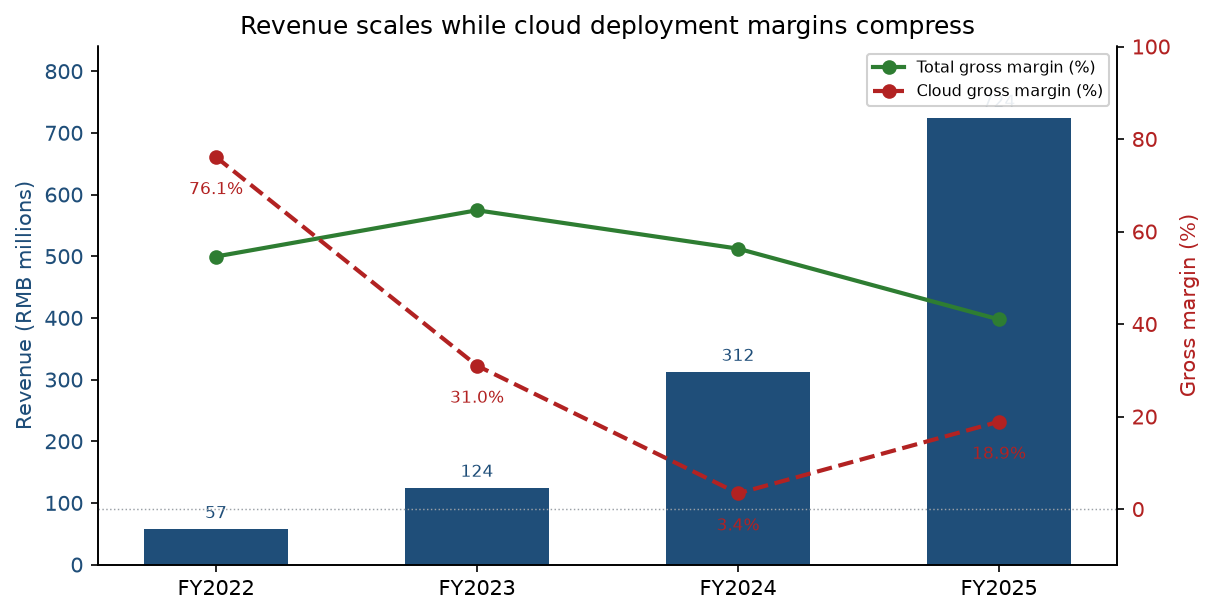
\includegraphics[width=\textwidth]{fig8_financial_profile.png}
    \end{column}
    \begin{column}{0.41\textwidth}
      \textbf{H1 2026 要看三件事}
      \begin{itemize}
        \item 半年收入 RMB 953.9m，已超过 FY2025 全年 RMB 724.3m。
        \item API 收入 RMB 825.2m，占比 86.5\%，同比增长 2,735.7\%。
        \item 毛利率由 50.0\% 降至 26.4\%，规模增长尚未转化为经营杠杆。
      \end{itemize}
      \smallnote{增长是真实的，单位经济性与费用强度同样真实；这正是估值分歧的来源。}
    \end{column}
  \end{columns}
\end{frame}

\begin{frame}{H1 2026：收入跃升，亏损仍是核心约束}
  \vspace{-0.3em}
  \begin{table}
    \centering
    \scriptsize
    \begin{tabular}{lrrr}
      \toprule
      RMB m & H1 2025 & H1 2026 & 同比变化 \\
      \midrule
      收入 & 190.9 & 953.9 & +399.7\% \\
      毛利 & 95.4 & 251.6 & +163.7\% \\
      经营亏损 & 1,899.2 & 2,146.6 & +13.0\% \\
      净亏损 & 2,357.9 & 2,072.0 & -12.1\% \\
      调整后亏损 & 1,752.0 & 1,964.1 & +12.1\% \\
      \bottomrule
    \end{tabular}
  \end{table}
  \smallnote{研发开支 RMB 2,131.2m，同比增长 33.6\%；净亏损收窄含金融工具公允价值变动影响，调整后亏损仍在扩大。}
  \begin{columns}[T,onlytextwidth]
    \begin{column}{0.48\textwidth}
      \textbf{资产负债表（2026-06-30）}
      \begin{itemize}
        \item 现金 RMB 3,993.7m；短期投资 RMB 506.1m。
        \item 银行借款 RMB 2,224.8m；租赁负债 RMB 379.4m。
      \end{itemize}
    \end{column}
    \begin{column}{0.48\textwidth}
      \textbf{读数边界}
      \begin{itemize}
        \item 7 月配售净募资 HK\$31.375bn，配售后股份 465.623m。
        \item 半年报于 8 月 31 日收市后发布，不能用来解释当日涨幅。
      \end{itemize}
    \end{column}
  \end{columns}
\end{frame}

\begin{frame}{模型发布节奏是论文的事件时间轴}
  \begin{columns}[T,onlytextwidth]
    \begin{column}{0.60\textwidth}
      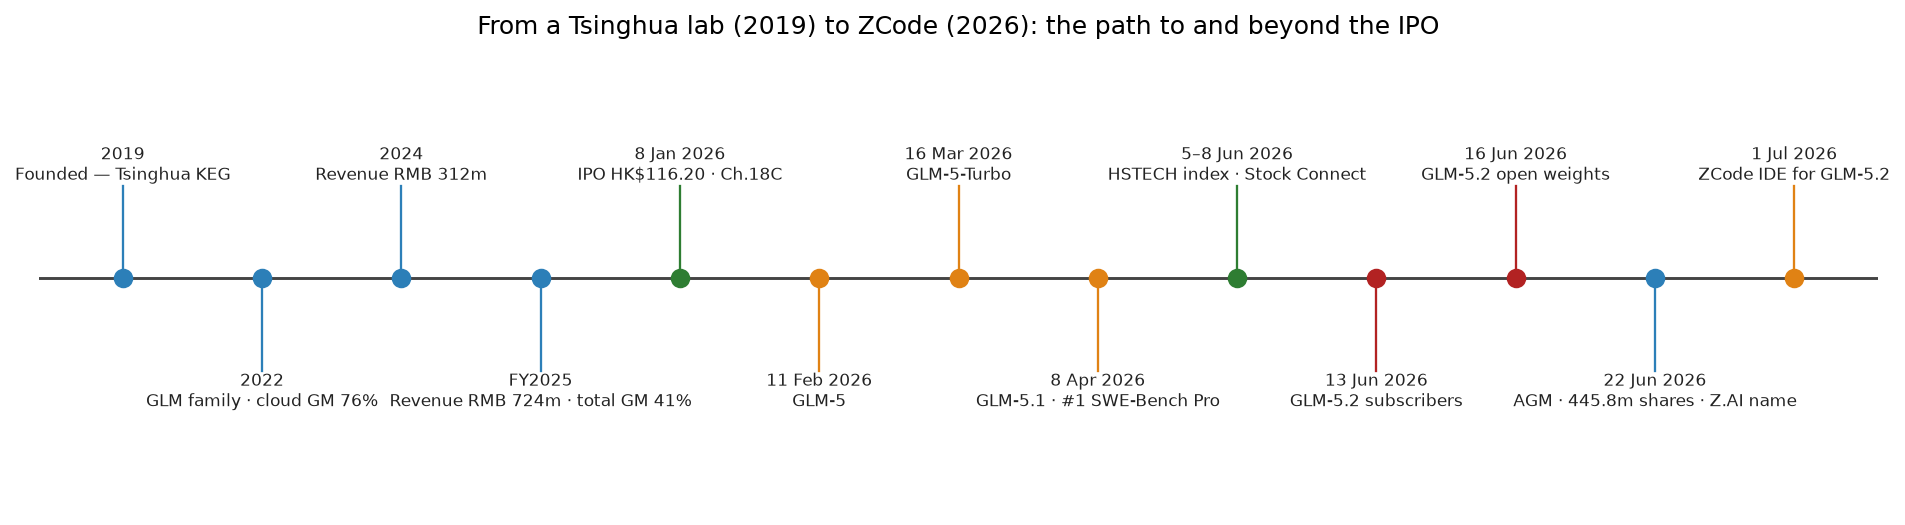
\includegraphics[width=\textwidth]{fig9_glm_timeline.png}
    \end{column}
    \begin{column}{0.36\textwidth}
      \textbf{为什么时间轴重要}
      \begin{itemize}
        \item GLM-5、Turbo、5.1、5.2、5.3 形成连续能力事件。
        \item 能力事件来自官方模型发布和 benchmark 变化，不从股价反推。
        \item 7 月配售和 8 月半年报另行归类，不和能力新闻混算。
        \item 这保证事件研究不是挑涨幅最大的日子。
      \end{itemize}
    \end{column}
  \end{columns}
\end{frame}

\begin{frame}{股价走势把估值问题推到极端}
  \centering
  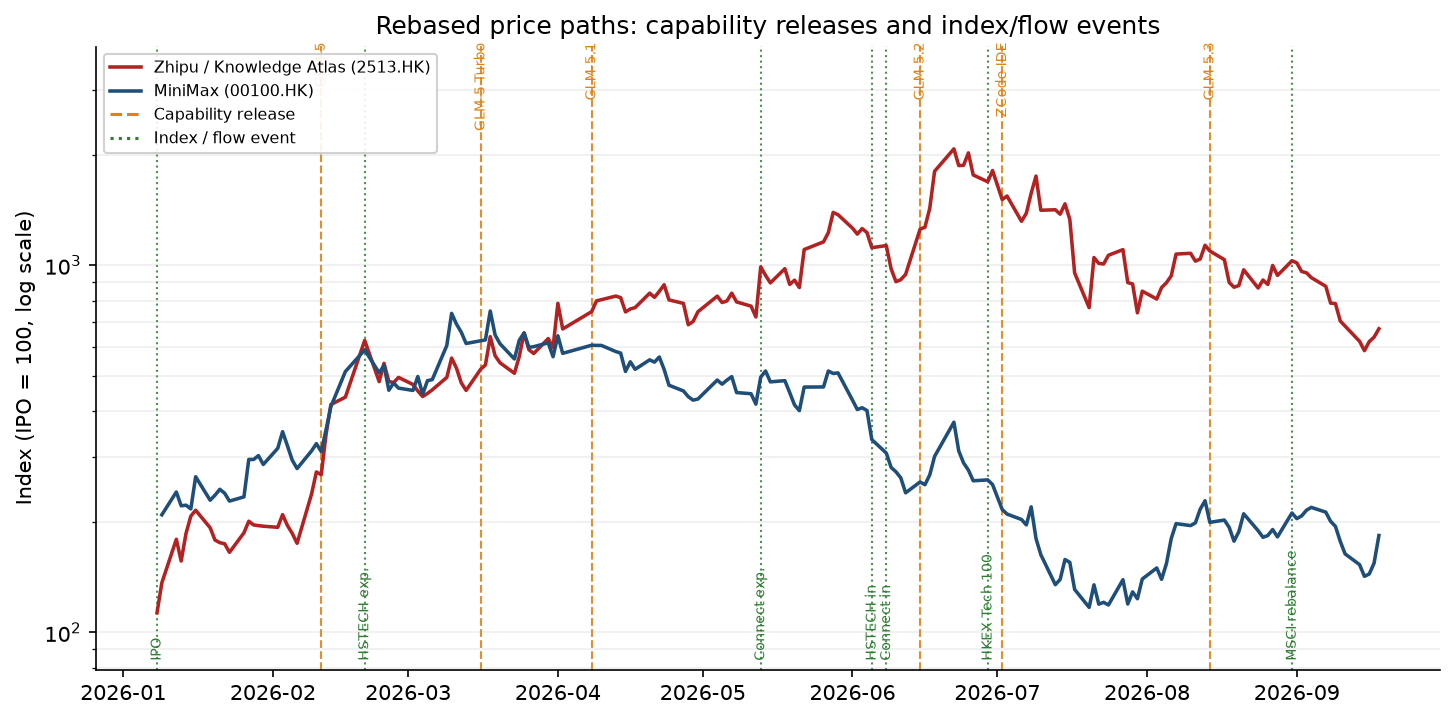
\includegraphics[height=0.66\textheight]{fig1_price_paths.png}
  \vspace{0.2em}
  \footnotesize
  截至 9 月 18 日，智谱较 IPO 上涨约 571\%，MiniMax 上涨约 84\%。8 月 31 日智谱收涨 9.6\%；半年报在收市后发布，不能解释这段涨幅，MSCI 月末再平衡则可能贡献了部分收盘资金流。
\end{frame}

\section{估值框架与隐含预期}

\begin{frame}{估值先从一个透明的 DCF 框架开始}
  \begin{columns}[T,onlytextwidth]
    \begin{column}{0.48\textwidth}
      \textbf{已披露事实与资金桥}
      \begin{itemize}
        \item H1 2026 收入 RMB 953.9m，经营利润率约 -225\%。
        \item 九月配售后股份 487.588m 股。
        \item 现金加短投、扣除借款与租赁，加七月与九月融资净款并扣除可转债本金代理值，pro forma 净现金约 US\$6.308bn。
      \end{itemize}
    \end{column}
    \begin{column}{0.48\textwidth}
      \textbf{模型假设，不是公司指引}
      \begin{itemize}
        \item FY2026E 收入 US\$700m。
        \item 起始经营利润率 -100\%，意味着 H2 经营效率显著改善。
        \item WACC 约 13.5\%，由 bottom-up beta 得到。
        \item 汇率假设：HK\$7.8/US\$，RMB 7.1/US\$。
      \end{itemize}
    \end{column}
  \end{columns}
  \smallnote{US\$6.308bn 为六月余额加后续融资并扣债的估值桥；不含未披露期后消耗，本金代理值并非公允价值。}
\end{frame}

\begin{frame}{DCF 的结果只解释了市价的一小部分}
  \vspace{-0.4em}
  \begin{table}
    \centering
    \scriptsize
    \begin{tabular}{lrrrr}
      \toprule
      情景 & 2035 收入 & EBIT margin & Equity value & 每股价值 \\
      & US\$bn & & US\$bn & HK\$ \\
      \midrule
      Bear & 4.4 & 18\% & 3.5 & 55.8 \\
      Base & 8.0 & 28\% & 6.4 & 101.8 \\
      Bull & 21.9 & 35\% & 15.9 & 254.9 \\
      \midrule
      概率加权 & -- & -- & 7.3 & 116.3 \\
      市场价格（9/18） & -- & -- & 48.8 & 780.0 \\
      \bottomrule
    \end{tabular}
  \end{table}
  \textbf{讲解重点：} 概率加权 DCF 约为市价的 14.9\%。这不是在宣告“正确价格”，而是在量化市场价格中有多少依赖尚未兑现的右尾结果。
\end{frame}

\begin{frame}{敏感性分析说明估值缺口不是小幅调参能解决}
  \begin{columns}[T,onlytextwidth]
    \begin{column}{0.58\textwidth}
      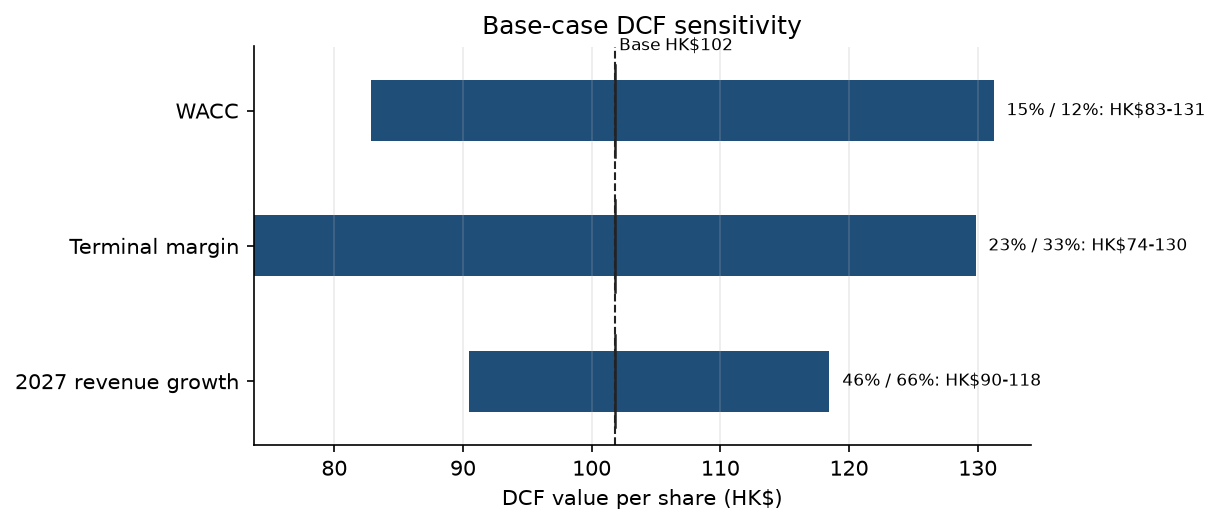
\includegraphics[width=\textwidth]{fig7_sensitivity.png}
    \end{column}
    \begin{column}{0.38\textwidth}
      \textbf{如何读这张图}
      \begin{itemize}
        \item 每个条形表示一个关键假设变化对每股价值的影响。
        \item 收入规模、长期利润率和 WACC 是最核心变量。
        \item 典型单变量区间约 HK\$74--131，仍难以靠常规调参接近 HK\$780。
      \end{itemize}
    \end{column}
  \end{columns}
\end{frame}

\begin{frame}{反向 DCF 把市场价格翻译成未来要求}
  \begin{columns}[T,onlytextwidth]
    \begin{column}{0.58\textwidth}
      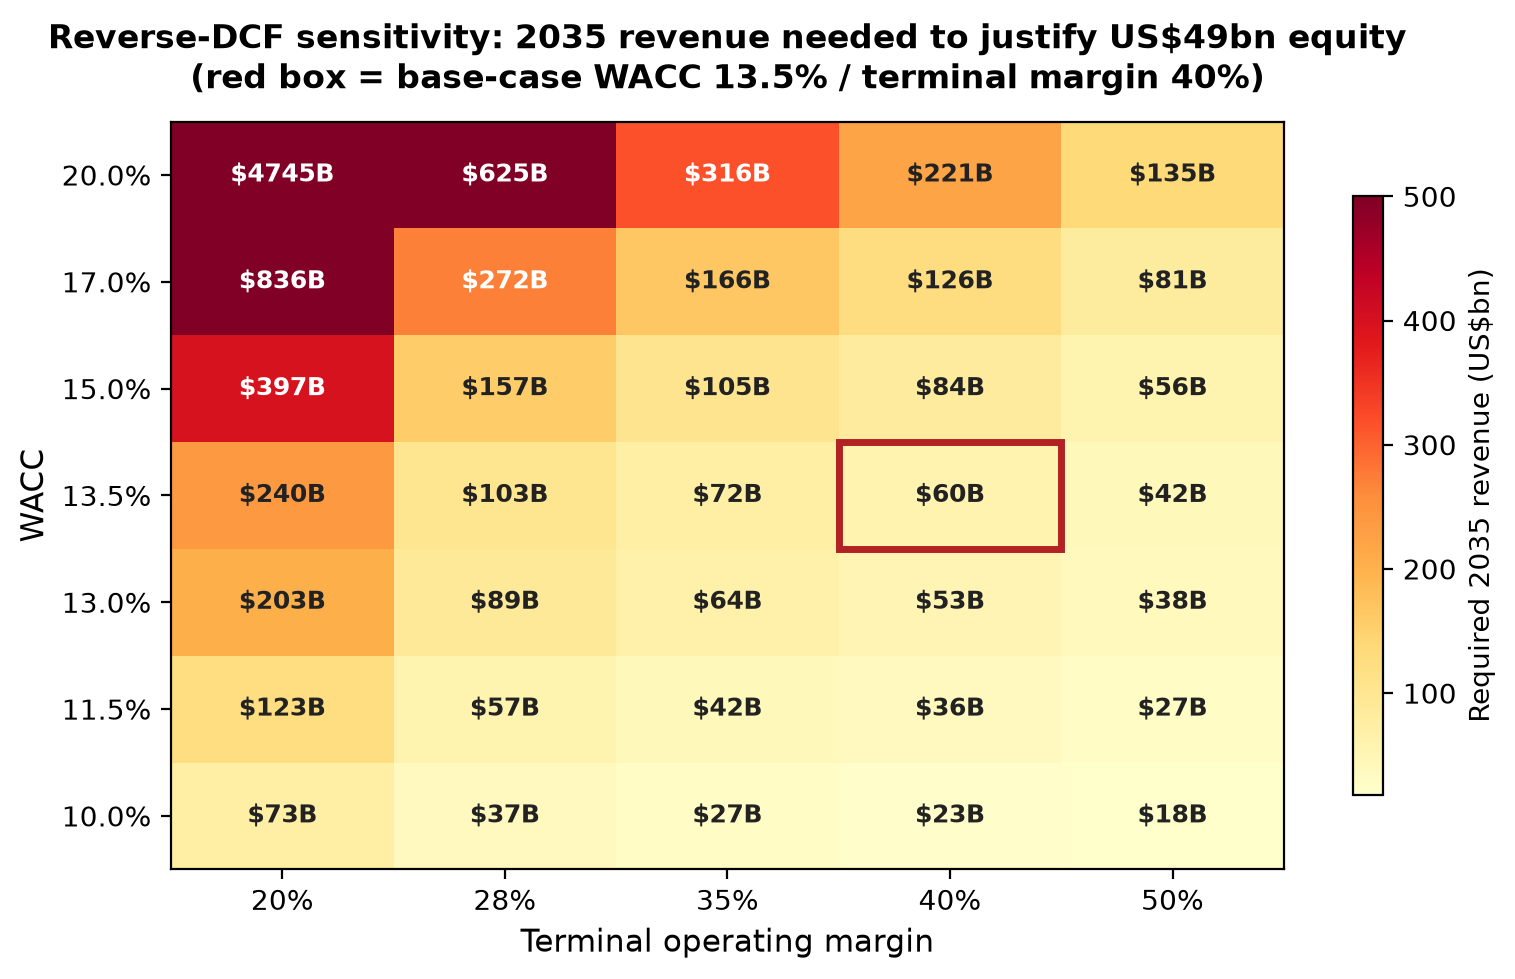
\includegraphics[width=\textwidth]{fig11_reverse_dcf_heatmap.png}
    \end{column}
    \begin{column}{0.38\textwidth}
      \textbf{关键读法}
      \begin{itemize}
        \item 横轴和纵轴分别改变终值利润率和 WACC。
        \item 每个格子显示要支撑 US\$48.8bn equity value 所需的 2035 年收入。
        \item 基准组合（13.5\% WACC、40\% 终值利润率）要求 2035 年收入 US\$59.7bn。
        \item 这相当于 2027 年增长 129.2\%，2026--2035 年 CAGR 63.9\%。
      \end{itemize}
      \smallnote{FY2026E 收入固定为 US\$700m；反向 DCF 求解的是此后增长路径。}
    \end{column}
  \end{columns}
\end{frame}

\begin{frame}{上市同行统一采用 LTM 收入口径}
  \begin{columns}[T,onlytextwidth]
    \begin{column}{0.58\textwidth}
      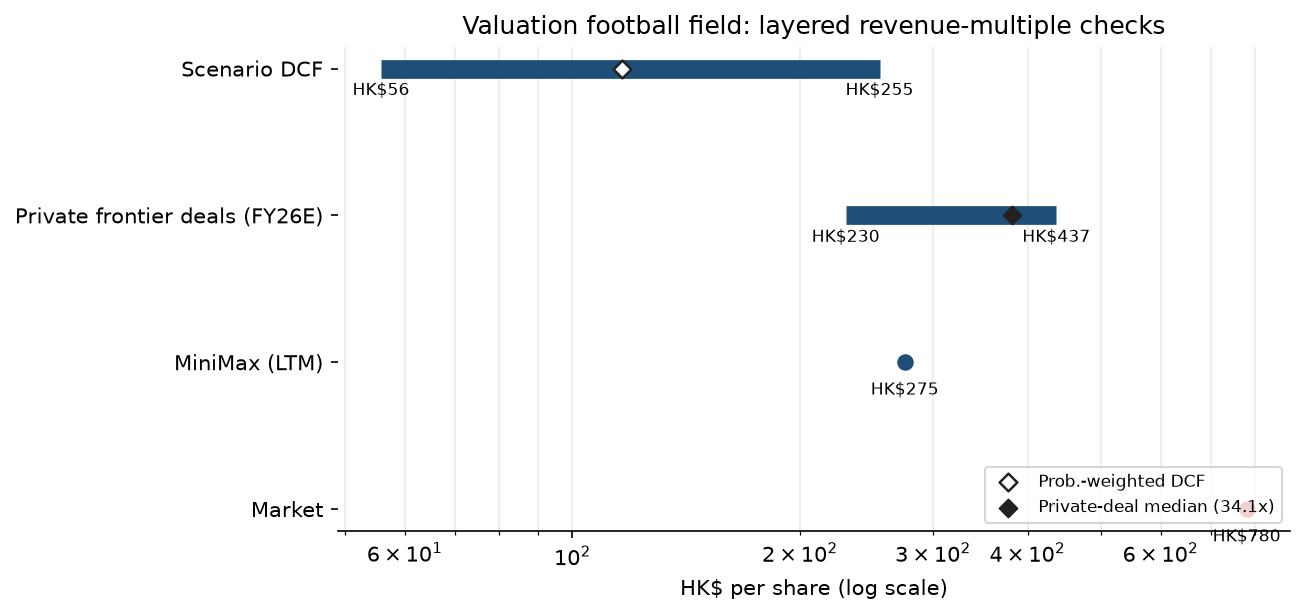
\includegraphics[width=\textwidth]{fig5_football_field.png}
    \end{column}
    \begin{column}{0.38\textwidth}
      \small
      \textbf{交叉验证}
      \begin{itemize}
        \item 私募基础模型交易区间为 20.5--39.0x，对应每股约 HK\$230--437。
        \item 智谱 LTM 收入 US\$209.5m，对应 232.8x；MiniMax 为 82.1x。
        \item MiniMax 倍数应用于智谱 LTM 收入，对应每股约 HK\$275。
      \end{itemize}
      \begin{block}{估值含义}
        两家上市公司都享有高估值，但智谱的收入倍数仍是 MiniMax 的 3.09 倍。
      \end{block}
    \end{column}
  \end{columns}
\end{frame}

\begin{frame}{三层可比回答三个不同的问题}
  \begin{columns}[T,onlytextwidth]
    \begin{column}{0.58\textwidth}
      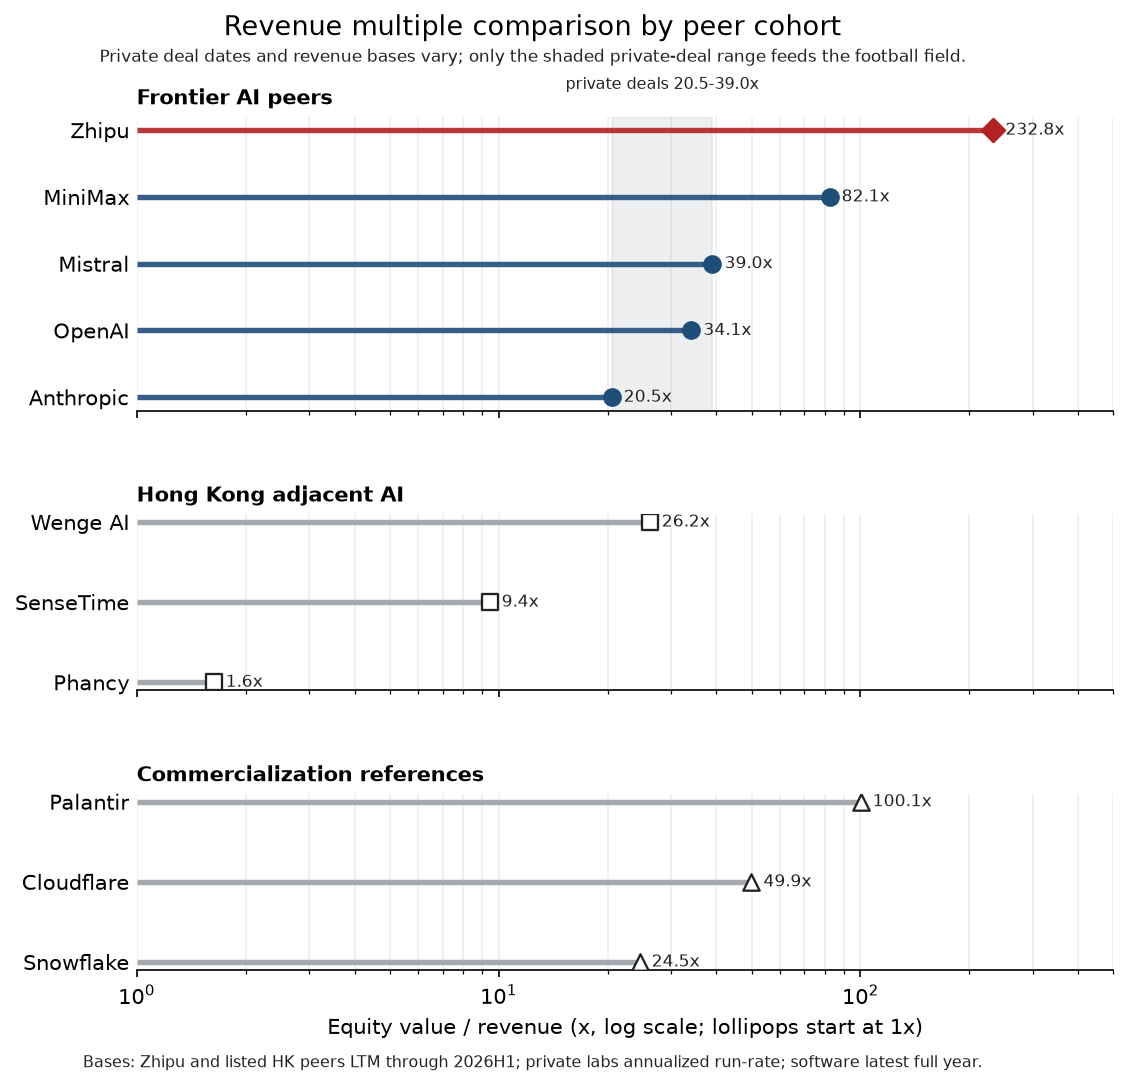
\includegraphics[width=\textwidth,height=0.68\textheight,keepaspectratio]{fig6_ps_comps.png}
    \end{column}
    \begin{column}{0.38\textwidth}
      \small
      \textbf{读图顺序}
      \begin{itemize}
        \item 上市基础模型同行采用同一 LTM 规则：智谱 232.8x，MiniMax 82.1x。
        \item 港股邻近组帮助判断本地 AI 资产的估值位置，但收入结构不同。
        \item 商业化参照组显示成熟 AI 软件的收入倍数，不参与核心中位数。
      \end{itemize}
      \smallnote{智谱倍数约为 MiniMax 的 3.09 倍。私募公司使用收入 run-rate，保留为单独的交易参照。}
    \end{column}
  \end{columns}
\end{frame}

\begin{frame}{实物期权解释把估值与事件研究连接起来}
  \begin{columns}[T,onlytextwidth]
    \begin{column}{0.48\textwidth}
      \textbf{现金流估值看到的公司}
      \begin{itemize}
        \item 早期收入基数小。
        \item 当前亏损大。
        \item 毛利率和算力成本不确定。
        \item 因此 DCF 的中位数价值很低。
      \end{itemize}
    \end{column}
    \begin{column}{0.48\textwidth}
      \textbf{期权视角看到的公司}
      \begin{itemize}
        \item 如果模型能力持续领先，平台化和 winner-take-all 概率上升。
        \item 能力突破会提高右尾 payoff 的概率。
        \item 能力停滞会迅速压缩期权价值。
      \end{itemize}
    \end{column}
  \end{columns}
  \vspace{0.5em}
  \begin{block}{自然过渡}
    如果市场买的是能力驱动的期权，那么真正要检验的是：能力新闻是否真的会移动股价。
  \end{block}
\end{frame}

\section{能力超预期事件研究}

\begin{frame}{传统 earnings surprise 不适合这类公司}
  \begin{columns}[T,onlytextwidth]
    \begin{column}{0.48\textwidth}
      \textbf{传统 PEAD 的逻辑}
      \begin{itemize}
        \item 公司公布盈利。
        \item 盈利高于或低于预期。
        \item 股价对盈利信息反应，并可能继续漂移。
      \end{itemize}
    \end{column}
    \begin{column}{0.48\textwidth}
      \textbf{智谱案例的问题}
      \begin{itemize}
        \item 盈利为负，且短期亏损主要反映投入强度。
        \item 市场更关心模型能力、开发者采用和未来平台化。
        \item 所以 surprise 的单位应从 earnings 换成 capability。
      \end{itemize}
    \end{column}
  \end{columns}
\end{frame}

\begin{frame}{事件研究设计尽量避免事后挑选}
  \begin{columns}[T,onlytextwidth]
    \begin{column}{0.48\textwidth}
      \textbf{事件分类}
      \begin{itemize}
        \item Capability：GLM 模型发布和 benchmark 跳升。
        \item Flow：HSTECH、Stock Connect、HKEX Tech 100、MSCI 等指数或资金流事件。
        \item Financial disclosure：半年报等财务披露，和模型能力分开识别。
        \item Listing：IPO 相关事件。
        \item Peer：MiniMax 的通用/旗舰模型事件；音乐、语音等垂类模型只保留在扩展目录中。
      \end{itemize}
    \end{column}
    \begin{column}{0.48\textwidth}
      \textbf{窗口与计算}
      \begin{itemize}
        \item 估计窗口：事件前局部非事件日。
        \item 泄露窗口：$[-5,-1]$。
        \item 反应窗口：$[0,+1]$。
        \item 漂移窗口：$[+2,+10]$。
      \end{itemize}
    \end{column}
  \end{columns}
  \smallnote{完整窗口样本含 16 个发行方自身可交易的 large-tech 发布；OpenAI/xAI 的股票代理、半年报及 8 月下旬不完整窗口只留目录，不强算 CAR。}
\end{frame}

\begin{frame}{五个 GLM 能力事件：四个原始短窗为正}
  \begin{table}
    \centering
    \small
    \begin{tabular}{lrrrr}
      \toprule
      事件 & 日期 & 反应 CAR & 漂移 CAR & Peer-adjusted 反应 \\
      \midrule
      GLM-5 & 2026-02-11 & +22.5\% & +24.7\% & +17.2\% \\
      GLM-5-Turbo & 2026-03-16 & +7.7\% & -19.3\% & +14.6\% \\
      GLM-5.1 & 2026-04-08 & +13.8\% & -14.2\% & +13.4\% \\
      GLM-5.2 & 2026-06-15 & +30.8\% & +28.2\% & +28.7\% \\
      GLM-5.3 & 2026-08-14 & -6.5\% & +3.8\% & +2.4\% \\
      \midrule
      平均 & -- & +13.7\% & +4.6\% & +15.3\% \\
      \bottomrule
    \end{tabular}
  \end{table}
  \begin{block}{结果含义}
    市场不是只买“AI 概念”：原始短窗 4/5 为正；以 MiniMax 调整后，5/5 均为正。
  \end{block}
\end{frame}

\begin{frame}{漂移结果更复杂，不能过度概括}
  \begin{columns}[T,onlytextwidth]
    \begin{column}{0.52\textwidth}
      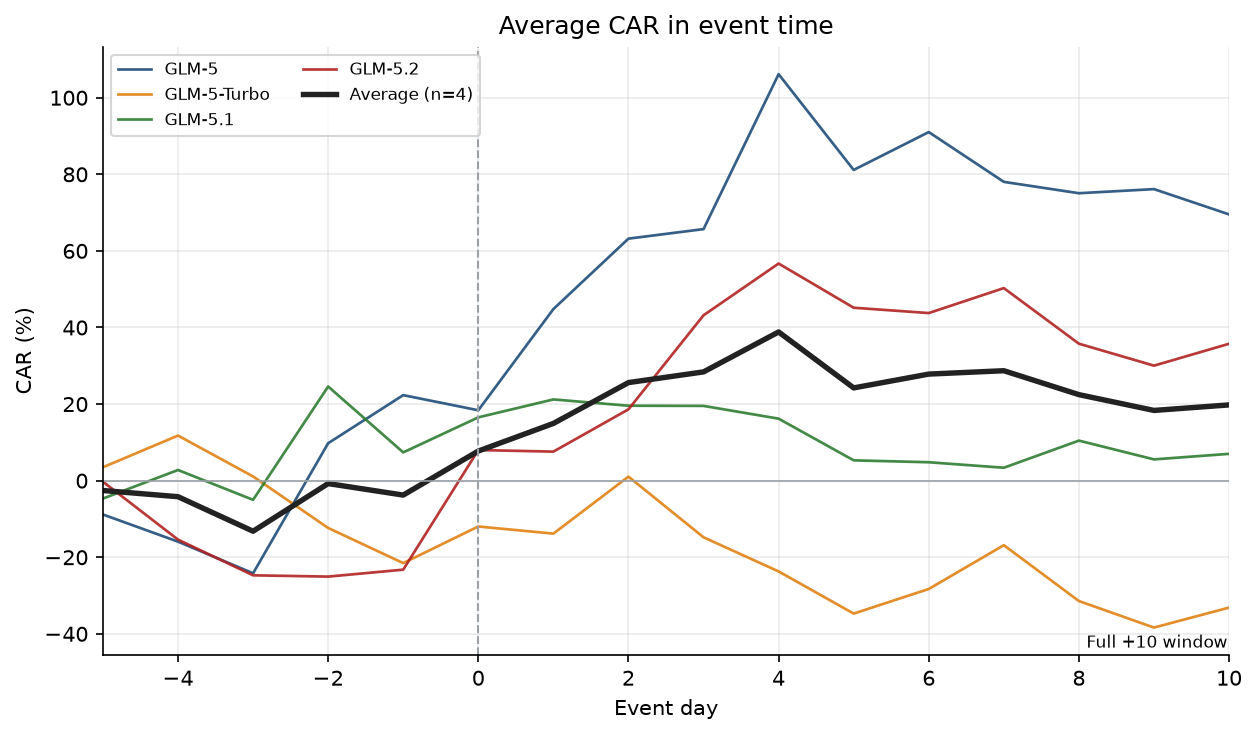
\includegraphics[width=\textwidth]{fig3_car_eventtime.png}
    \end{column}
    \begin{column}{0.44\textwidth}
      \textbf{图上的信息}
      \begin{itemize}
        \item 平均事件时间 CAR 在短窗快速上行。
        \item 漂移平均为正，但单个事件分化明显。
        \item GLM-5 与 GLM-5.2 更强；GLM-5.3 发布前已有明显预期交易。
      \end{itemize}
      \begin{block}{论文边界}
        这支持 PCAD 的案例证据，但不等同于大样本定律。
      \end{block}
    \end{column}
  \end{columns}
\end{frame}

\begin{frame}{资金流事件解释了部分尖峰，但不是能力证据}
  \begin{columns}[T,onlytextwidth]
    \begin{column}{0.49\textwidth}
      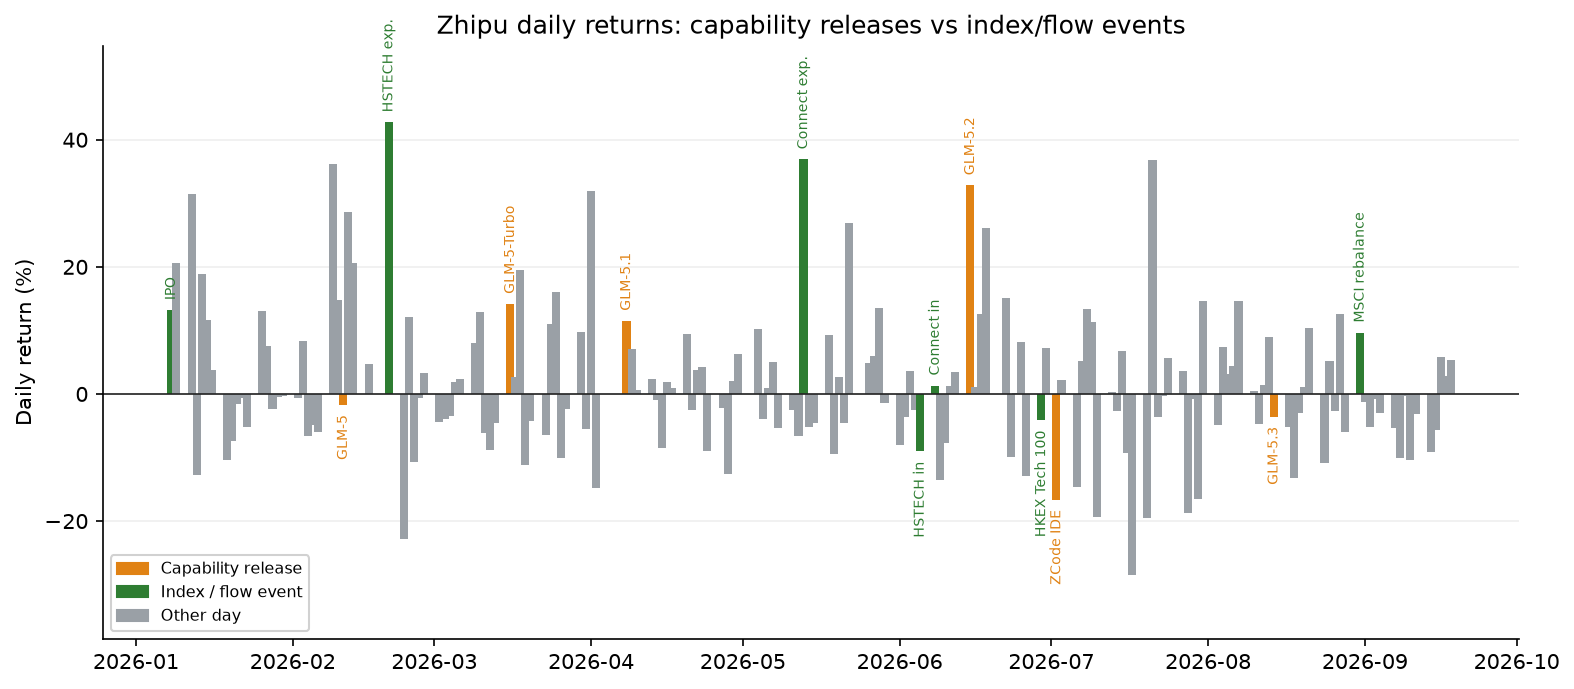
\includegraphics[width=\textwidth]{fig2_daily_returns.png}
    \end{column}
    \begin{column}{0.49\textwidth}
      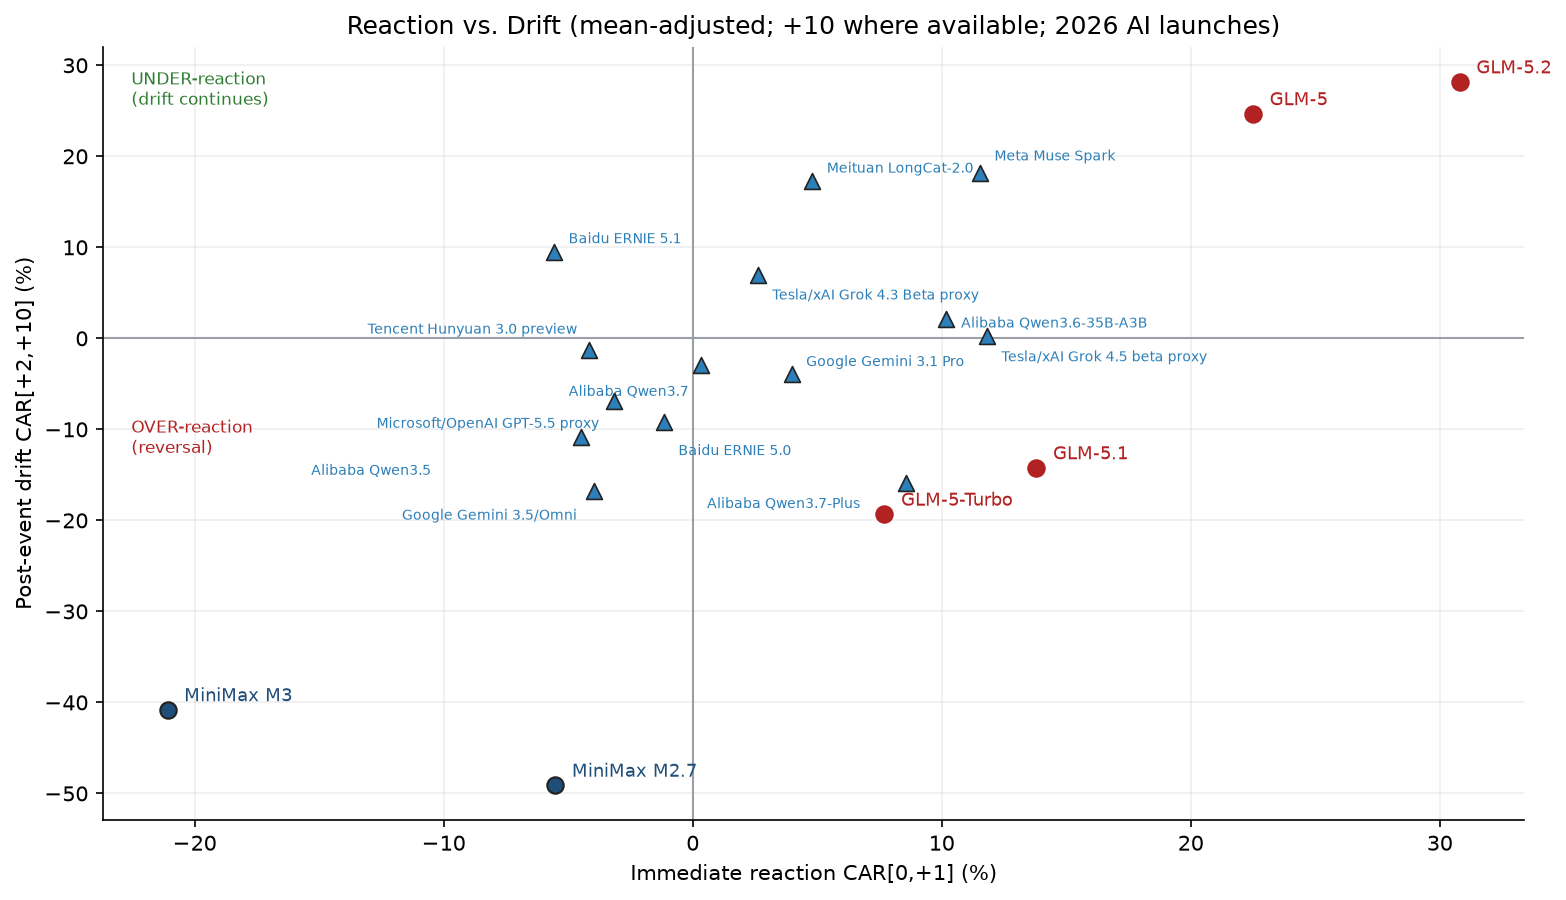
\includegraphics[width=\textwidth]{fig4_reaction_vs_drift.png}
    \end{column}
  \end{columns}
  \vspace{0.3em}
  \footnotesize
  最大日收益并不一定来自模型发布。2 月和 5 月的尖峰更多对应 HSTECH 与 Stock Connect 预期；8 月 31 日收涨 9.6\% 时，半年报尚未发布，MSCI 收盘再平衡则与交易时点重合。把流动性催化剂单独归类，才能避免把资金流误读为能力进步。
\end{frame}

\begin{frame}{MiniMax 对照帮助区分公司能力和板块情绪}
  \begin{columns}[T,onlytextwidth]
    \begin{column}{0.48\textwidth}
      \textbf{为什么需要 peer-adjusted}
      \begin{itemize}
        \item AI 板块可能整体上涨。
        \item 港股科技股可能同时受资金流影响。
        \item MiniMax 是同期香港上市的最接近公开市场对照。
      \end{itemize}
    \end{column}
    \begin{column}{0.48\textwidth}
      \textbf{对照后的结果}
      \begin{itemize}
        \item 五个 GLM 事件的平均 peer-adjusted 反应为 +15.3\%，漂移为 +16.8\%。
        \item MiniMax M2.5 反应为 +24.2\%，但 M2.7 与 M3 均为负反应/负漂移，说明市场并非奖励每次升级。
        \item 这说明市场在区分模型质量，而不是简单买入“AI lab”标签。
      \end{itemize}
    \end{column}
  \end{columns}
\end{frame}

\begin{frame}{Bootstrap 说明短窗反应较强，漂移证据较弱}
  \begin{columns}[T,onlytextwidth]
    \begin{column}{0.58\textwidth}
      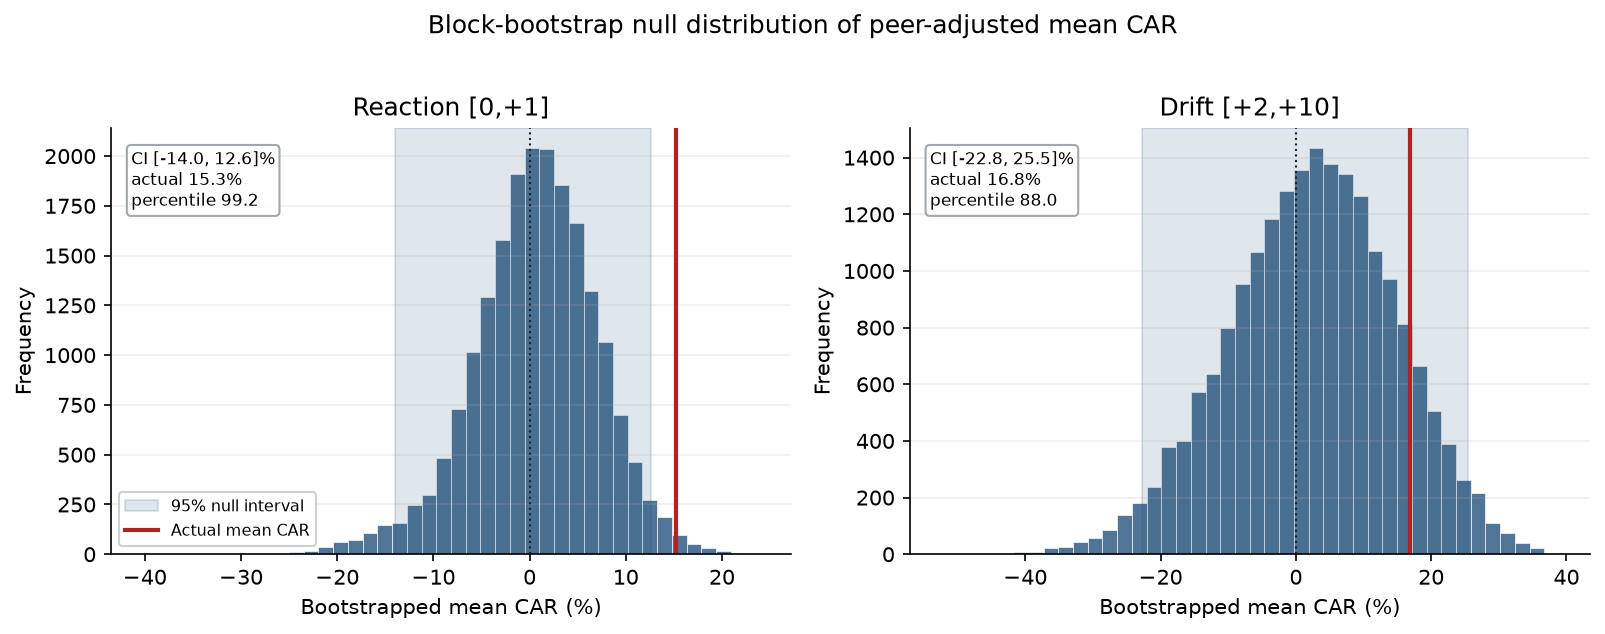
\includegraphics[width=\textwidth]{fig10_block_bootstrap.png}
    \end{column}
    \begin{column}{0.38\textwidth}
      \textbf{如何解释}
      \begin{itemize}
        \item 样本只有五个 GLM 事件，不能做夸张的参数检验。
        \item block bootstrap 用非事件窗口构造 null distribution。
        \item 实际短窗反应高于 95\% null 区间；漂移只属于方向性证据。
      \end{itemize}
    \end{column}
  \end{columns}
\end{frame}

\section{综合判断与答辩口径}

\begin{frame}{论文把估值缺口和事件反应合在一起解释}
  \begin{columns}[T,onlytextwidth]
    \begin{column}{0.48\textwidth}
      \textbf{如果只看估值}
      \begin{itemize}
        \item 结论会变成：市场价远高于基本面。
        \item 但这无法解释为什么能力发布日会有系统反应。
      \end{itemize}
    \end{column}
    \begin{column}{0.48\textwidth}
      \textbf{如果只看事件}
      \begin{itemize}
        \item 结论会变成：市场重视模型能力。
        \item 但这无法说明当前价格需要多极端的未来。
      \end{itemize}
    \end{column}
  \end{columns}
  \vspace{0.5em}
  \begin{block}{合并后的判断}
    能力进展解释早期重估，亏损和资金需求约束溢价；本周产品信任争议使商业化质量更重要。
  \end{block}
\end{frame}

\begin{frame}{投资含义是同时跟踪财务与能力两只时钟}
  \begin{columns}[T,onlytextwidth]
    \begin{column}{0.32\textwidth}
      \textbf{对投资者}
      \begin{itemize}
        \item 区分模型能力事件和资金流事件。
        \item 用半年报检验收入质量、毛利率与费用杠杆。
        \item 用能力日历跟踪 benchmark、价格策略和开发者采用。
        \item 对高估值保持止损纪律。
      \end{itemize}
    \end{column}
    \begin{column}{0.32\textwidth}
      \textbf{对公司}
      \begin{itemize}
        \item 能力发布是资本市场的核心沟通货币。
        \item API 已成为主收入来源且自身毛利率转正；总毛利率因收入结构变化而下降。
        \item 开源低价策略需要证明可变现。
      \end{itemize}
    \end{column}
    \begin{column}{0.32\textwidth}
      \textbf{对市场制度}
      \begin{itemize}
        \item Chapter 18C 让预盈利科技公司更早进入公开市场。
        \item 公开市场需要学习如何定价技术能力。
        \item 信息披露应更重视技术里程碑。
      \end{itemize}
    \end{column}
  \end{columns}
\end{frame}

\begin{frame}{答辩时最可能被追问的三点}
  \begin{columns}[T,onlytextwidth]
    \begin{column}{0.32\textwidth}
      \textbf{DCF 是否太保守}
      \begin{itemize}
        \item FY2026E 收入 US\$700m 已远高于 H1 年化水平。
        \item -100\% 起始利润率也假设 H2 较 H1 的 -225\% 显著改善。
        \item 即便如此，反向 DCF 仍显示市价要求极端增长路径。
      \end{itemize}
    \end{column}
    \begin{column}{0.32\textwidth}
      \textbf{样本是否太小}
      \begin{itemize}
        \item 承认样本小。
        \item 因此论文只声称诊断性证据。
        \item 用 peer-adjusted 和 bootstrap 降低误读。
      \end{itemize}
    \end{column}
    \begin{column}{0.32\textwidth}
      \textbf{为什么不是纯泡沫}
      \begin{itemize}
        \item 稳定正反应说明市场至少会分辨能力新闻。
        \item MiniMax 的 82.1x 倍数显示板块有共同溢价，但远低于智谱的 232.8x。
        \item 但小样本事件研究不能排除泡沫，高估值仍可能快速回撤。
      \end{itemize}
    \end{column}
  \end{columns}
\end{frame}

\begin{frame}{本周先跌后弹，不能把均值回归写成单边下跌}
  \begin{itemize}
    \item 智谱：9/11 HK\$793，周二 HK\$680，周五 HK\$780；周跌 1.64\%。
    \item MiniMax：9/11 HK\$270，周二 HK\$234.6，周五 HK\$303；周涨 12.22\%。
    \item 周五分别上涨 5.41\% 与 18.92\%；8 月底以来仍回撤 34.7\% 与 13.2\%。
    \item 原五事件与 bootstrap 固定在 8 月 31 日，新增消息分开登记。
    \item 智谱财报九日漂移现完整，为 -54.35\%；窗口重叠，不能视为孤立因果。
  \end{itemize}
  \smallnote{11 条日线均截至 9 月 18 日；季度现金消耗尚未披露。均值回归是对预期溢价部分压缩的描述。}
\end{frame}

\begin{frame}{融资已完成：同时更新现金、债务与股本}
  \begin{itemize}
    \item 配售 2,196.5 万股于 9/16 完成；HK\$714/股，净款 HK\$156.64 亿。
    \item 可转债于 9/18 发行；净款 US\$30.11 亿，本金 RMB201.4 亿、美元结算。
    \item 现有股本 4.876 亿股；全额初始转股后约 5.140 亿股。
    \item 初始转股价 HK\$892.50，2027 年 9 月到期；零息仍有偿债义务。
  \end{itemize}
  \begin{block}{本期估值口径}
    净现金桥约 US\$63.08 亿，扣除约 US\$30.01 亿发行时点本金代理值；未转股口径的加权 DCF 为 HK\$116。变化来自融资，经营预测未提高。
  \end{block}
  \smallnote{来源：9/18 港交所完成公告。本金代理值 = 美元总款 / 100.5\%，非公允价值；不含未知现金消耗。}
\end{frame}

\begin{frame}{闻歌半年业绩：收入增长与亏损改善的成色}
  \begin{itemize}
    \item 收入 RMB1.728 亿，同比 +46.0\%；毛利率 55.0\%（去年 54.6\%）。
    \item 部署收入占 65.9\%；订阅及 API 占 34.1\%，后者同比 +94.0\%。
    \item 总亏损 RMB8,765 万，收窄 24.5\%；归母亏损收窄 27.6\%。
    \item 经调整亏损 RMB5,292 万，收窄 29.5\%；研发费用增长 59.0\%。
    \item 金融资产公允价值收益 RMB3,505 万，亦帮助报表亏损收窄。
  \end{itemize}
  \begin{block}{可比性判断}
    部署模式仍占主导，继续作为邻近可比。现金等价物升至 RMB10.18 亿，流动性增长主要来自 IPO，不能据此认定经营现金流转正。
  \end{block}
  \smallnote{来源：闻歌 8 月 25 日中期业绩公告；金额为人民币。原可比表已使用 H1 更新的 LTM 收入。}
\end{frame}

\begin{frame}{ZCode 争议：客户信任进入商业化风险}
  \begin{itemize}
    \item 开发者指控工作区及 Git 历史被打包上传，UI 开关不能有效阻断。
    \item 周五 15:32 已有报道；争议并非只在盘后出现。
    \item 19:48 报道转述官方致歉：称索引/Repo Wiki 导致上传，问题已修复。
    \item 官方称生成 Wiki 后数据销毁，并承诺开源和第三方审查。
  \end{itemize}
  \begin{block}{对估值意味着什么}
    信任可能影响留存、企业采购和修复成本。指控尚未经本文复现，删除和修复是公司说法；不能声称所有代码已泄露或用于训练，也不能凭空估计损失。
  \end{block}
  \smallnote{来源：ferstar 原始分析、ChooseAI 时间记录、IT之家。排除 9/19 新增版本复核，区分指控与回应。}
\end{frame}

\begin{frame}{MiniMax Code CLI 开源的是工具层}
  \begin{itemize}
    \item 官方仓库 v0.4.12、MIT 许可：终端编码 Agent 的源码可审查、修改。
    \item 可读写项目、执行命令和测试，支持自带模型；不是基础模型权重开源。
    \item 不同于较早的 MiniMax 通用多模态 CLI，也不等于整个桌面端开放。
    \item 透明度可降低企业评估门槛，但不自动证明安全或收入增长。
  \end{itemize}
  \begin{block}{股价归因必须遵守时序}
    第一财经 20:39 报道正式开放，晚于周五 +18.92\% 的收盘涨幅。报道未必是首次传播；截至本期无后续交易日，不将当天上涨写成晚间报道的反应。
  \end{block}
  \smallnote{来源：MiniMax 官方 9/18 GitHub 快照与第一财经。同样不将智谱 +5.41\% 归因于晚间回应。}
\end{frame}

\begin{frame}{最后的结论}
  \begin{block}{一句话}
    能力超预期推动重估，随后预期溢价部分回归；本周反弹与分化显示调整并非单向。融资能力、产品信任和持续变现共同决定每股价值。
  \end{block}
  \vspace{0.4em}
  \textbf{论文的三个贡献}
  \begin{itemize}
    \item 把半年报、配售与市场价格拆成事实，再把预测明确标成模型假设。
    \item 用 DCF、可比估值和反向 DCF 明确市价所要求的未来。
    \item 用 capability surprise 替代 earnings surprise，适配早期基础模型公司。
  \end{itemize}
  \vspace{0.5em}
  \centering
  {\large \textbf{Capability repricing, partial reversion, and product trust}}
\end{frame}

\end{document}
